\chapter{Akustické vlastnosti Makoňova korpusu}
\label{kap:akustika}

Mluvený korpus Karla Makoně vyniká vzhledem ke své velikosti konzistencí téměř
výlučně jediného mluvčího a velmi úzkou tematickou doménou. Jistou protiváhu
této konsistentnosti představují jeho akustické vlastnosti.

\section{Výchozí akustická kvalita}

Akustická kvalita nahrávek je největší slabinou korpusu. Kvalita není
konzistentně špatná, je velmi kolísavá. Na kvalitu záznamu má vliv jeho stáří,
použité médium, rychlost záznamu, způsob skladování, zda se jedná o
originál\footnote{kopírování magnetofonových pásek je ztrátový proces}, použitý
magnetofon, mikrofon, pozice mikrofonu, akustické vlastnosti prostředí jako
ozvěna, hluk na pozadí, ale také momentální dispozice mluvčího.

Obrázky~\ref{fig:spectr-ok} až~\ref{fig:spectr-fasttalk} ukazují spektrogramy
nahrávek různých kvalit. Vždy se jedná přibližně o třísekundový úsek a součástí
popisku je odkaz pro přehrání odpovídajícího zvuku.

\begin{figure}[htpb]
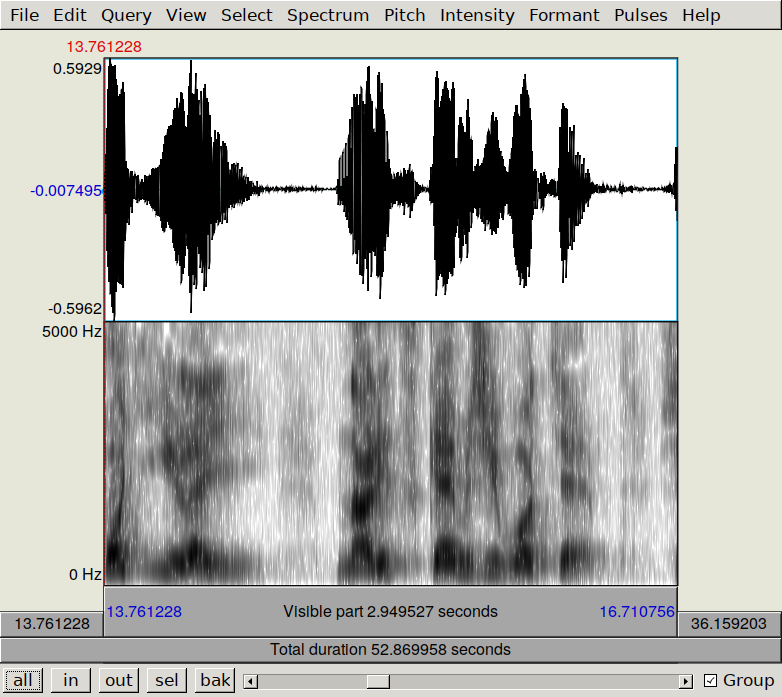
\includegraphics[scale=0.89]{rc/spectrum-dobry-90-02A.png}
\caption{
    kvalitní záznam bez zjevných defektů\\
    \texttt{http://radio.makon.cz/zaznam/90-02A\#ts=673.14}
}
\label{fig:spectr-ok}
\end{figure}

\begin{figure}[htpb]
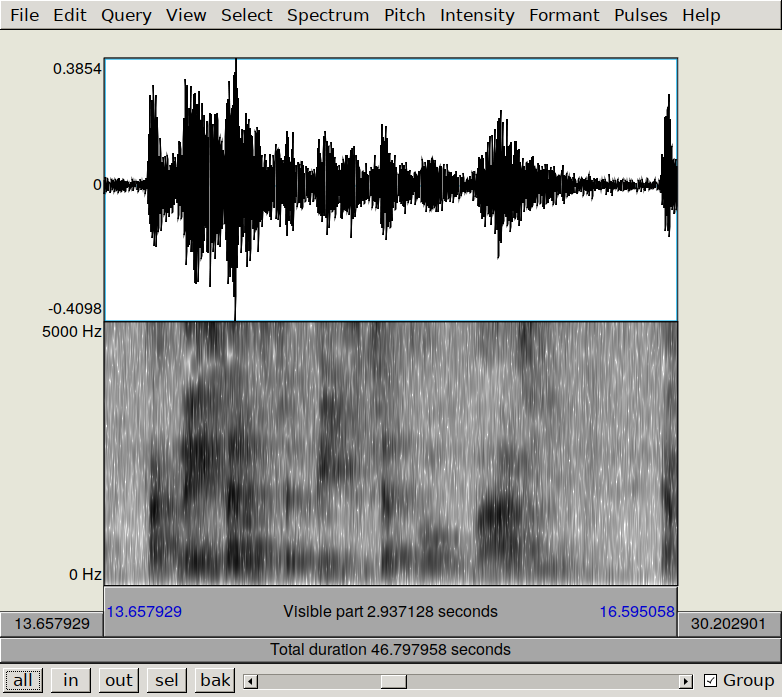
\includegraphics[scale=0.89]{rc/spectrum-echo-90-24A.png}
\caption{
    výrazné echo\\
    \texttt{http://radio.makon.cz/zaznam/90-24A-24.4.90\#ts=664.33}
}
\label{fig:spectr-echo}
\end{figure}

\begin{figure}[htpb]
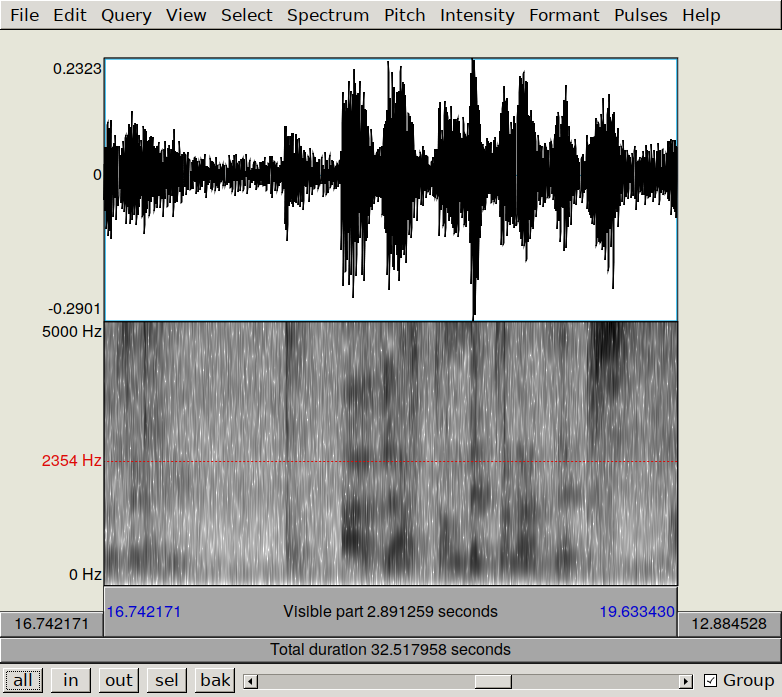
\includegraphics[scale=0.89]{rc/spectrum-noise-92-04A.png}
\caption{
    širokopásmový šum\\
    \texttt{http://radio.makon.cz/zaznam/92-04A\#ts=691.37}
}
\label{fig:spectr-noise}
\end{figure}

\begin{figure}[htpb]
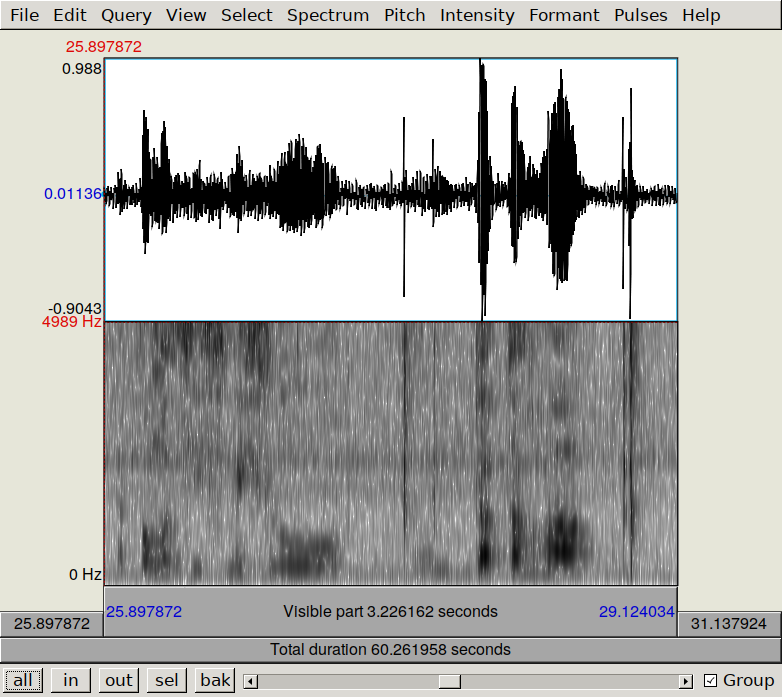
\includegraphics[scale=0.89]{rc/spectrum-narrow-92-03B.png}
\caption{
    úzkopásmový šum\\
    \texttt{http://radio.makon.cz/zaznam/92-03B\#ts=664.43}
}
\label{fig:spectr-narrow}
\end{figure}

\begin{figure}[htpb]
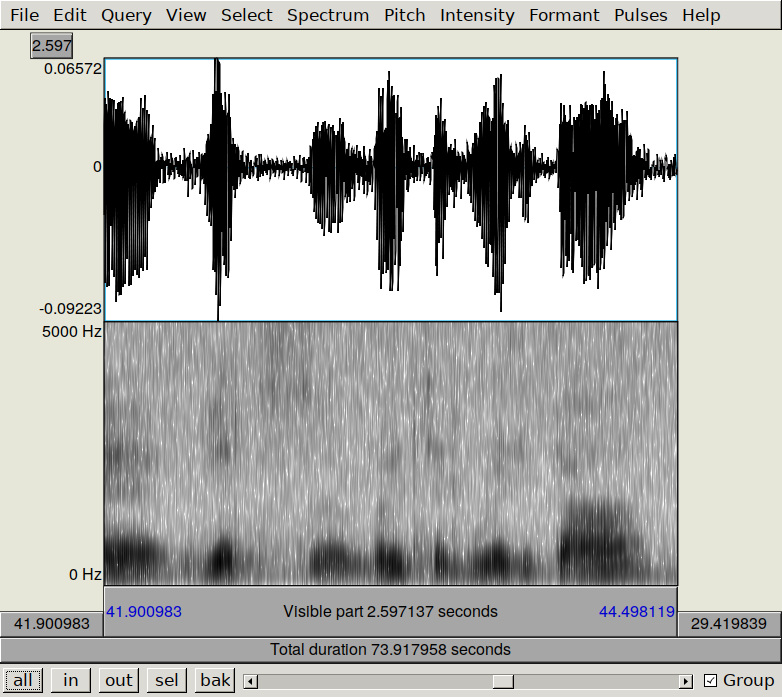
\includegraphics[scale=0.89]{rc/spectrum-nohighs-88-04A.png}
\caption{
    absence vysokých frekvencí\\
    \texttt{http://radio.makon.cz/zaznam/88-04A\#ts=678.94}
}
\label{fig:spectr-nohi}
\end{figure}

%\begin{figure}[htpb]
%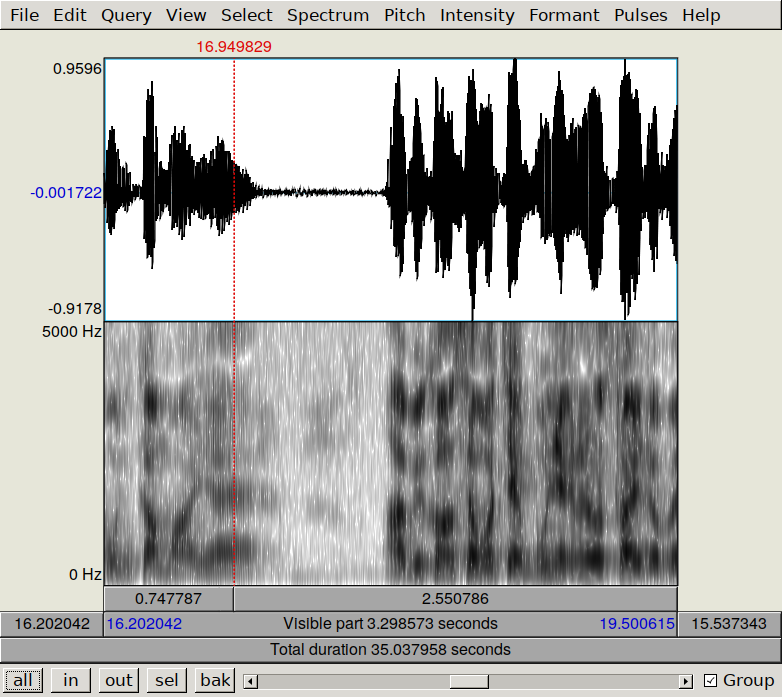
\includegraphics[scale=0.89]{rc/spectrum-overdrive-91-20A.png}
%\caption{
%    přebuzení
%    \texttt{http://radio.makon.cz/zaznam/91-20A\#ts=600.00}
%}
%\label{fig:spectr-overdrive}
%\end{figure}

\begin{figure}[htpb]
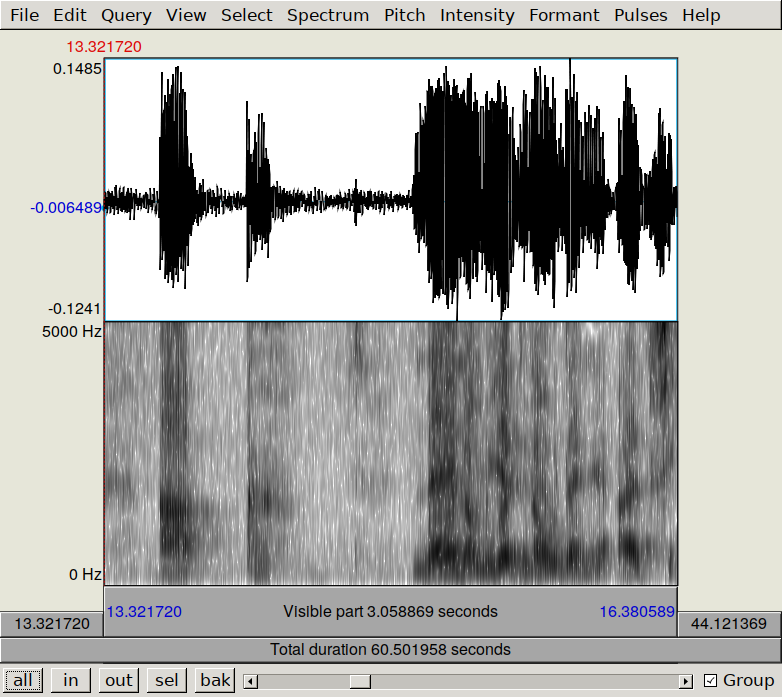
\includegraphics[scale=0.89]{rc/spectrum-accel-90-18A.png}
\caption{
    zrychlený záznam způsobený zpomalením převíjení pásky při nahrávání\\
    \texttt{http://radio.makon.cz/zaznam/90-18A-XX-zrychlene\#ts=2473.56}
}
\label{fig:spectr-accel}
\end{figure}

\begin{figure}[htpb]
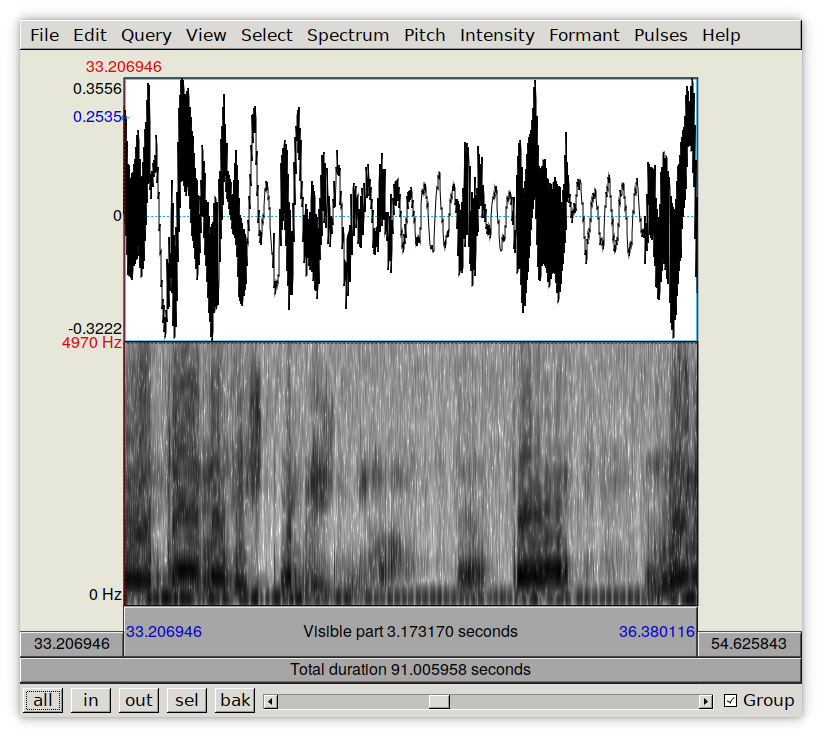
\includegraphics[scale=0.89]{rc/spectrum-2cms-ktplzneid01a.png}
\caption{
    silně degradovaná nahrávka pořízená rychlostí 2,38 cm/s\\
    \texttt{http://radio.makon.cz/zaznam/kotouc-plzen-neident01-a\#ts=660}
}
\label{fig:spectr-2cms}
\end{figure}

\begin{figure}[htpb]
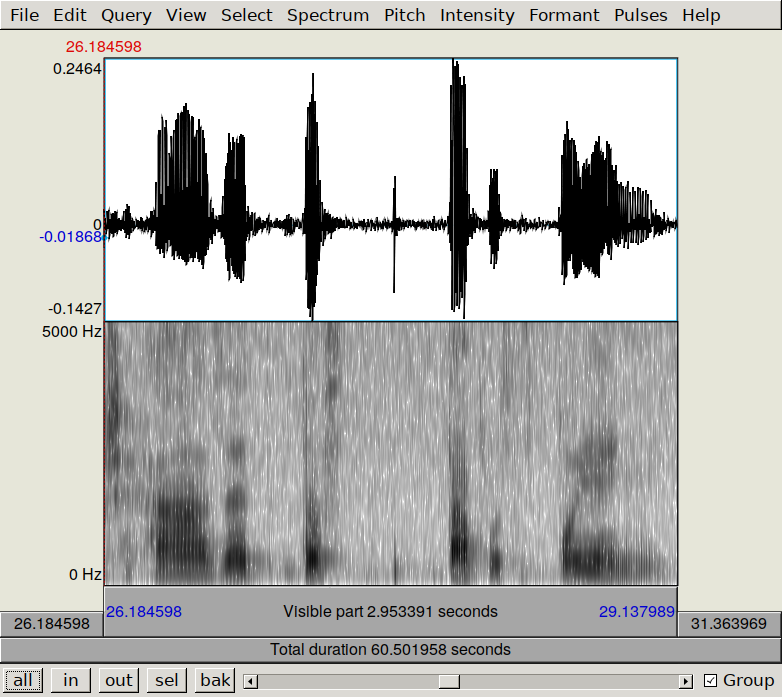
\includegraphics[scale=0.89]{rc/spectrum-pomala-mluva-76-04A.png}
\caption{
    pomalá mluva\\
    \texttt{http://radio.makon.cz/zaznam/76-04A-Kaly-7-IEOUA\#ts=13.79}
}
\label{fig:spectr-slowtalk}
\end{figure}

\begin{figure}[htpb]
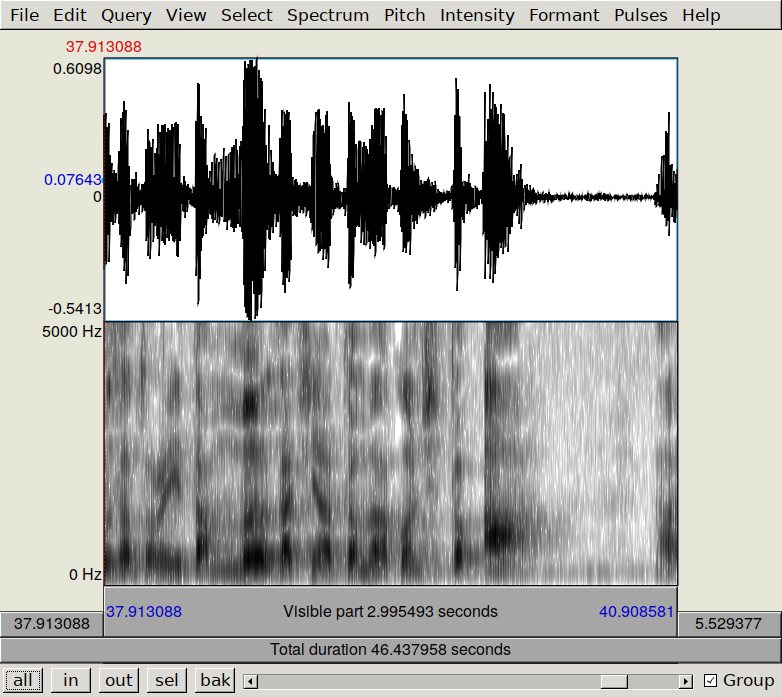
\includegraphics[scale=0.89]{rc/spectrum-rychla-mluva-89-11B.png}
\caption{
    rychlá mluva\\
    \texttt{http://radio.makon.cz/zaznam/89-11B\#ts=203.17}
}
\label{fig:spectr-fasttalk}
\end{figure}

\section{Kompenzace akustických vad}

\subsection{Metrika}

Předpokladem pro práci s~akustickými vlastnostmi dat je porovnávání na jejich
základě. Je tedy nutné mít metriku, která by odrážela akustickou podobnost
jednotlivých souborů. K~tomu využívám algoritmu založeného na koeficientech
MFCC, jak to navrhují Mandel a Ellis (2005)\cite{mandel2005song}. Využívám
k~tomu programu Musly od Dominka Schnitzera (2011)\cite{schnitzer2011using}.

V~rámci nahrávek dochází často ke změnám akustických vlastností. To je dáno
hlavně tím, že se nahrávání uprostřed pásky přerušilo a obnovilo se v~jiných
podmínkách. Není proto žádoucí porovnávat celé nahrávky. Ideální by bylo
detekovat akustické zlomy v~nahrávkách a korpus přerozdělit ne podle hranic
nahrávek, ale podle těchto zlomů.

Pro jednoduchost jsem nahrávky rozdělil do menších úseků a udělal matici
akustické vzdálenosti na nich. Pokusil jsem se využít hotových úseků rozdělených
v~bodech ticha, viz sekci~\ref{sec:segmenty}. Výsledná matice o rozměrech
80~000 \times 80~000 však trpěla defekty při čtení a zápisu, proto jsem velikost
úseků pro tento účel zvětšil na 10 minut a tím dosáhl počtu 8146 úseků.

Pro orientaci uvedu některé údaje z~matice podobnosti. 
Medián vzdálenosti je 55,8.
Maximální vzdálenost je $3,40\cdot{}10^{38}$, ovšem ta nastává v~okrajových
případech, bez zjevného důvodu patrného lidskému uchu. Bez této astronomické
maximální vzdálenosti dosahují vzdálenosti hodnot do 27~814.
Počet nulových vzdáleností je 275 z~celkových 33~174~585.



Abychom tato čísla mohli interpretovat, porovnejme je se vzdálenostmi jiných
zvuků, které si snad čtenář dokáže představit.

Ku příkladu tři různí mluvčí jednoho záznamu jednání poslanecké sněmovny
parlamentu České republiky mají vzdálenost v rozmezí 6,5 a 9,5. Dva různé úseky
téhož mluvčího mají vzdálenost 1,4. Tyto záznamy z PSP ČR jsou i pro lidské ucho
velmi podobné a na rozdílu ve vzdálenosti mezi různými mluvčími a v~rámci
mluvčího je vidět, že algoritmus funguje dobře.

Jako druhý příklad vezměme typickou, úsměvně známou ukázku mluveného slova
s~hlukem na pozadí, a sice úryvek ,,to je dost, žes nás taky jednou vyvez, žes
udělal něco pro rodinu`` z~filmu Slavnosti sněženek. Jednotliví mluvčí (Blažena
Holišová a Rudolf Hrušínský) mají vzájemnou vzdálenost 13,9. Holišová od
samotného malotraktoru 48,2 a Hrušínský od téhož 23,7.

Vzdálenost mezi úryvky ze Slavností sněženek a PSP ČR se pohybují mezi 31,8 a
127,9. Konkrétně Holišová má od Okamury vzdálenost 31,8 a samotný malotraktor od
Okamury 127,9.

Jako třetí příklad uvedu dvě skladby z~populární hudby: Billie Jean od Michaela
Jacksona, která je zvukově celou dobu téměř neměnná (což nic neubírá na její
kvalitě) a skladbu Shadow Sun od metalové skupiny Moonspell. Ta je žánrově od
Billie Jean velmi vzdálená a obsahuje velice různorodé pasáže. Vzdálenost celých
skladeb od sebe je 48,3. Vzdálenost sloky a refrénu v~rámci Shadow Sun je 46,5,
vzdálenost refrénu Shadow Sun od Billie Jean je 299,0 a vzdálenost sloky Shadow
Sun od Billie Jean je 47,4.

Vzdálenost hudebních úseků od poslanců se pohybuje od 23,1 (Jackson X
Sklenák) do 519 (refrén Shadow Sun X Tomio Okamura). Vzdálenost hudebních
úseků od Slavností sněženek se pohybuje od 27,0 (Jackson X Holišová) do 311
(refrén Shadow Sun X malotraktor).

Je tedy patrno, že akustická variabilita korpusu Karla Makoně je i podle tohoto
měřítka obrovská.

\section{Shlukování}

Kompenzovat akustické nedostatky znamená měnit akustické kvality dat tak, aby
lépe odpovídaly nějakému kritériu. To může být subjektivní: aby se zvuk určitému
posluchači lépe poslouchal. Může být také objektivní, strojově vyhodnotitelné,
což pak umožní nasazení strojových metod.

V~korpusu Karla Makoně se nevyskytuje asi žádná nahrávka ve vysoké kvalitě
srovnatelné s~materiálem pořízeným ve studiových podmínkách. Velká část
nahrávek, obzvlášť kazety z~let 1984 a dál, jsou veskrze srozumitelné a bez
zásadních defektů. Z~celého korpusu jsem vybral množinu 431 souboru v~uspokojivé
kvalitě.

Tato referenční množina je mnohem konzistentnější co do akustické metriky než
celý korpus, ale v~porovnání s~ilustračními příklady mimo korpus stále řádově
divergentnější. Vzdálenosti se pohybují od 1,6 do 14~653 s~průměrem  54,7 a
mediánem 9,40.

Na množině úseků, které jsem porovnával akustickou metrikou, jsem provedl
hierarchické shlukování. Vzdálenost clusteru jsem nastavil jako maximální
vzdálenost mezi dvěma prvky, aby jednotlivé clustery byly co nejkompaktnější.

\section{Kompenzace}

Expertní manuální odstranění by bylo ideálním postupem pro získání nejlepšího
možného výsledku, ale stejně jako v případě přepisu je pro velikost korpusu
nedostupný. Krom toho je manuální čištění řemeslem, které neovládám.

Jaké jsou možnosti automatického akustického zdokonalování signálu?

% >>> np.mean(a)
% 54.730708459073007
% >>> np.median(a)
% 9.3979599999999994
